\documentclass[10pt,aspectratio=169]{beamer}

\usepackage[T1]{fontenc}
\usepackage{lmodern}
\usepackage{amsmath,amssymb,mathtools,booktabs,array,graphicx,microtype}
\usepackage{appendixnumberbeamer}

% Classic Copenhagen/whale seminar style, matching the research/pow decks.
\usetheme{Copenhagen}
\usecolortheme{whale}
\usefonttheme{professionalfonts}
\usefonttheme{serif}
\setbeamertemplate{navigation symbols}{}
\setbeamertemplate{itemize items}[circle]
\setbeamertemplate{blocks}[default]
\setbeamertemplate{headline}{}
\setbeamertemplate{footline}{%
  \begin{beamercolorbox}[wd=\paperwidth,ht=2.5ex,dp=1.1ex,leftskip=1em,rightskip=1em]{author in head/foot}%
    \usebeamerfont{author in head/foot}\insertshorttitle\hfill\insertframenumber/\inserttotalframenumber
  \end{beamercolorbox}%
}

\definecolor{paperblue}{HTML}{1D409E}
\definecolor{paperorange}{HTML}{D55E00}
\definecolor{paperteal}{HTML}{009E73}
\definecolor{papergray}{HTML}{66717E}
\definecolor{paperink}{HTML}{20252B}
\definecolor{paperlight}{HTML}{EAF1F8}
\setbeamercolor{normal text}{fg=paperink,bg=white}
\setbeamercolor{alerted text}{fg=paperblue}
\setbeamercolor{frametitle}{fg=white,bg=paperblue}
\setbeamercolor{title}{fg=white}
\setbeamercolor{subtitle}{fg=paperlight}
\setbeamercolor{structure}{fg=paperblue}
\setbeamercolor{palette primary}{fg=white,bg=paperblue}
\setbeamercolor{palette secondary}{fg=white,bg=paperblue!85!black}
\setbeamercolor{palette tertiary}{fg=white,bg=paperblue!70!black}
\setbeamercolor{author in head/foot}{fg=white,bg=paperblue!85!black}
\setbeamercolor{block title}{fg=paperblue,bg=paperblue!9}
\setbeamercolor{block body}{fg=paperink,bg=paperblue!4}
\setbeamercolor{alertblock title}{fg=white,bg=paperblue!88!black}
\setbeamercolor{alertblock body}{fg=paperink,bg=paperblue!6}
\setbeamerfont{title}{size=\LARGE,series=\bfseries}
\setbeamerfont{subtitle}{size=\large,series=\mdseries}
\setbeamerfont{frametitle}{size=\large,series=\bfseries}
\setbeamerfont{caption}{size=\scriptsize}
\setlength{\parskip}{0.2em}

\title[Deployment Utility of a Frozen Policy-Update Procedure]{Evaluating the Deployment Utility of a Frozen Policy-Update Procedure:\\Scale, Completion Preference, and Joint Evidence}
\subtitle{Research Presentation}
\author{}
\date{}

\begin{document}

% Frame 1: Title
\begin{frame}
  \titlepage
  \vspace{-1.0em}
  \begin{block}{Scope of This Study}
    \footnotesize
    Empirical and methodological evaluation of one frozen replay-proxy policy-update procedure in a controlled synthetic continuous double auction, using saved outcomes, root-level inference, and explicit distinctions between confirmatory and post-outcome diagnostics.
  \end{block}
\end{frame}

% Frame 2: Why proxy scores are insufficient
\begin{frame}{Why Proxy Scores Are Insufficient for Deployment Assessment}
  \begin{itemize}
    \item Candidate policy updates are frequently screened on cheap replay or proxy benchmarks before interactive deployment.
    \item A positive proxy gain does not guarantee positive incumbent-relative utility once the selected policy interacts with an active environment.
    \item Four distinct mechanisms can separate proxy screening from deployed utility:
      \begin{enumerate}
        \item \textbf{Winner selection:} choosing among multiple candidates induces selection optimism on finite proxy samples.
        \item \textbf{Interactive feedback:} deployed orders alter book state, liquidity, and subsequent fills unlike passive replay.
        \item \textbf{Operating scale:} order size changes market impact and execution completion rates.
        \item \textbf{Completion preferences:} deployment utility depends on how incomplete fills are penalized relative to execution prices.
      \end{enumerate}
    \item Sign-reversal frequency alone is insufficient: deployment value depends on the magnitudes of gains and losses, including no-update decisions.
  \end{itemize}
\end{frame}

% Frame 3: Procedure-level estimand and research questions
\begin{frame}{Procedure-Level Estimand and Research Questions}
  \footnotesize
  \begin{block}{Formal Target (Procedure-Level Deployment Utility)}
    Expected incumbent-relative utility of the \emph{complete frozen procedure}---retaining both candidate adoption and no-update decisions---under declared operating conditions, candidate-generation population, utility function, and joint evidence family.
  \end{block}

  \vspace{0.3em}
  \textbf{What this paper does not propose:}
  \begin{itemize}
    \item No new off-policy estimator, fidelity metric, selection algorithm, or universal deployment theorem.
  \end{itemize}

  \vspace{0.3em}
  \textbf{Primary Research Questions:}
  \begin{enumerate}
    \item \textbf{Operating scale \& liquidity:} How does deployed incumbent-relative utility vary across order scales ($s \in \{0.002, 0.05, 0.3\}$), liquidity regimes (liquid, thin), and inventory responses ($\rho \in \{0,1\}$)?
    \item \textbf{Utility and evidence sensitivity:} How does fixed-selection revaluation across incomplete-fill penalties ($p \in \{25, 50, 100, 200\}$ bps), together with the choice of inferential family, change the deployment assessment?
  \end{enumerate}
  \vspace{0.2em}
  \small\emph{Auxiliary diagnostic:} a separate post-outcome proxy-to-deployment comparison is reported at the selection scale ($s=0.05$); it is not a primary research question.
\end{frame}

% Frame 4: Relationship to prior work
\begin{frame}{Related Work and Scope Boundary}
  \scriptsize
  \renewcommand{\arraystretch}{1.12}
  \begin{tabular}{@{}p{0.28\textwidth}p{0.68\textwidth}@{}}
    \toprule
    \textbf{Research Area} & \textbf{Relationship and Boundary to This Work} \\
    \midrule
    Off-Policy Evaluation (OPE) \& High-Confidence OPE & Evaluates policies from logged data. We evaluate paired interactive deployments of a frozen replay-screened update procedure. \\
    \addlinespace[0.3em]
    Safe Policy Improvement (SPIBB) & Constructs safer policy improvements under uncertainty. We audit a fixed procedure without altering its selection rule. \\
    \addlinespace[0.3em]
    Conservative Evaluation of Offline Policy Learning & Close TMLR precedent on rigorous evaluation of offline learning pipelines. We focus on procedure-level deployment utility across scale and penalty preferences. \\
    \addlinespace[0.3em]
    Active Offline Policy Selection & Adaptively allocates limited online evaluation budgets across candidates. Here, selection is frozen on replay proxies prior to deployment assessment. \\
    \addlinespace[0.3em]
    HAL \& Agent Reliability & Studies system-level benchmarking and ranking measurement. We evaluate a specific frozen market-execution update procedure. \\
    \addlinespace[0.3em]
    PIVOT (Improvement Fidelity \& PIVOT-KG) & Studies transition-level Improvement Fidelity and PIVOT-KG. This paper evaluates frozen procedure-level deployment utility and does not replace those methods or repeat PIVOT results. \\
    \bottomrule
  \end{tabular}
\end{frame}

% Frame 5: First formal characterization
\begin{frame}{Formal Characterization 1: Reversal Accounting}
  \small
  \emph{These are elementary formal characterizations, not new estimators or deep general theorems.}
  \vspace{0.35em}
  \begin{block}{Gain and loss magnitudes matter}
    Let $A$ denote adoption; an incumbent-retaining decision has zero procedure gain. Then
    \[
      \mathbb{E}[\Delta U] = \Pr(A)\!\left[\Pr(\Delta U\geq0\mid A)\mathbb{E}[\Delta U\mid A,\Delta U\geq0]
      -\Pr(\Delta U<0\mid A)\mathbb{E}[|\Delta U|\mid A,\Delta U<0]\right].
    \]
  \end{block}
  \vspace{0.4em}
  \begin{alertblock}{Interpretation}
    Adoption or reversal frequency alone cannot determine procedure value. Two procedures can have the same reversal rate but opposite means when their positive and negative outcome magnitudes differ.
  \end{alertblock}
  \vfill
  \centering\scriptsize The estimand retains no-update decisions; it is not the mean of adopted updates only.
\end{frame}

% Frame 6: Second and third formal characterizations
\begin{frame}{Formal Characterizations 2--3: Utility and Sampling}
  \footnotesize
  \begin{block}{2. Fixed-selection completion-utility frontier}
    For the same selected policies and deployments, separating the execution component $a$ from completion shortfall $b$ gives
    \[
      \mu(p)=a+p\,b.
    \]
    A mathematical zero, when $b\neq0$, is $p^*=-a/b$. Changing $p$ does not reselect candidates.
  \end{block}
  \vspace{0.25em}
  \begin{block}{3. Root/deployment variance decomposition}
    For $R$ independent roots and $m$ repeated deployments per root,
    \[
      \operatorname{Var}(\widehat\mu)=\frac{\operatorname{Var}_R(g_R)}{R}+\frac{\mathbb{E}_R[\sigma_R^2]}{R m}.
    \]
    More repetitions reduce within-root deployment noise; only more independent roots reduce root-population variation.
  \end{block}
  \begin{alertblock}{Why it matters here}
    The 2,400 paired deployment records improve within-root precision, but the primary independent unit remains the 50-root cluster.
  \end{alertblock}
\end{frame}

% Frame 7: Frozen protocol and independent units
\begin{frame}{Frozen Experimental Protocol and Statistical Units}
  \footnotesize
  \begin{columns}[T,onlytextwidth]
    \begin{column}{0.52\textwidth}
      \textbf{Frozen selection and evaluation design}
      \begin{itemize}\itemsep0.25em\parskip0pt
        \item \textbf{Environment:} Synthetic continuous double auction.
        \item \textbf{Procedure:} One frozen replay-proxy policy-update procedure.
        \item \textbf{Generation roots:} $50$ independent generation roots; each root screens $16$ candidate policies.
        \item \textbf{Selection decisions:} $100$ root--regime selection decisions: one for each of $50$ roots in each liquidity regime.
        \item \textbf{Interactive evaluation:} $2{,}400$ paired interactive deployment records; selected policies and incumbents are evaluated on separate interactive books.
      \end{itemize}
    \end{column}
    \begin{column}{0.45\textwidth}
      \textbf{Operating grid and confirmatory family}
      \begin{itemize}\itemsep0.25em\parskip0pt
        \item \textbf{Liquidity regimes:} Liquid and thin.
        \item \textbf{Order scales:} $s \in \{0.002,\; 0.05,\; 0.3\}$.
        \item \textbf{Inventory response:} $\rho \in \{0,\; 1\}$.
        \item \textbf{Confirmatory utility:} $U_{100}$ with a $100$-bps incomplete-fill penalty.
        \item \textbf{Multiplicity control:} Approximate simultaneous confidence band over a prespecified $24$-estimate confirmatory family.
      \end{itemize}
      \vspace{0.2em}
      \begin{block}{Independent unit of inference}
        The independent statistical unit is the \textbf{root} ($R=50$), not each deployment record. Repeated deployments reduce within-root noise without adding new roots.
      \end{block}
    \end{column}
  \end{columns}
\end{frame}

% Frame 8: Main scale results
\begin{frame}{Main Scale Results Under $U_{100}$}
  \begin{columns}[c]
    \begin{column}{0.53\textwidth}
      \centering
      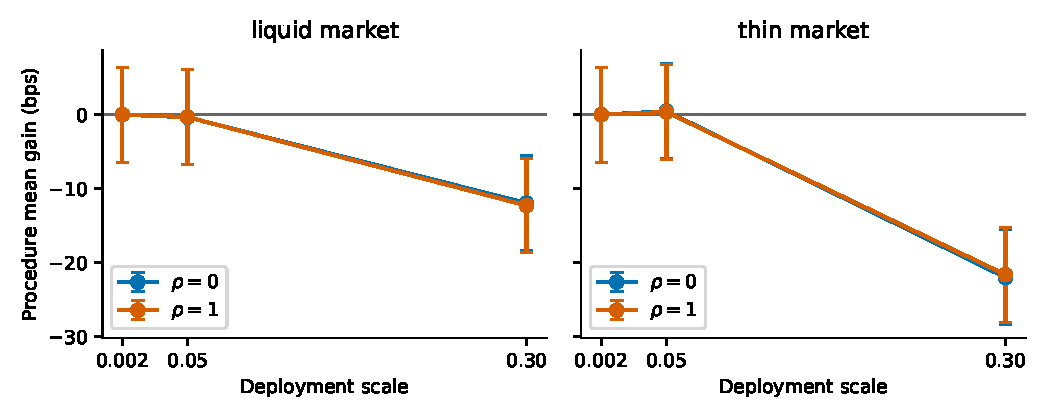
\includegraphics[width=\textwidth,height=0.68\textheight,keepaspectratio]{market_scale.pdf}
    \end{column}
    \begin{column}{0.45\textwidth}
      \small
      \textbf{Largest-Scale ($s=0.3$) Cell Means (bps)}\\
      {\footnotesize Original $24$-estimate simultaneous intervals:}
      \vspace{0.4em}

      \resizebox{\linewidth}{!}{%
      \begin{tabular}{@{}lrr@{}}
        \toprule
        \textbf{Cell ($s=0.3$)} & \textbf{Mean} & \textbf{Simultaneous CI} \\
        \midrule
        Liquid, $\rho=0$ & $-11.9800$ & $[-18.3944, -5.5656]$ \\
        Liquid, $\rho=1$ & $-12.2848$ & $[-18.6992, -5.8704]$ \\
        Thin, $\rho=0$   & $-22.0073$ & $[-28.4217, -15.5929]$ \\
        Thin, $\rho=1$   & $-21.6446$ & $[-28.0590, -15.2302]$ \\
        \bottomrule
      \end{tabular}
      }

      \vspace{0.6em}
      \begin{itemize}
        \item At $s=0.3$, all four regime-by-response cells exhibit clearly negative incumbent-relative deployment utility.
        \item Thin liquidity doubles the magnitude of the largest-scale loss relative to liquid books.
      \end{itemize}
    \end{column}
  \end{columns}
\end{frame}

% Frame 9: What the 24-estimate joint family supports
\begin{frame}{What the Prespecified 24-Estimate Joint Family Supports}
  \begin{columns}[T]
    \begin{column}{0.48\textwidth}
      \begin{block}{Supported by Original Joint Family}
        \begin{itemize}
          \item Negative incumbent-relative deployment utility under $U_{100}$ at the largest order scale ($s=0.3$) in all four operating cells:
            \begin{itemize}
              \item Liquid, $\rho=0$: $-11.9800$ bps
              \item Liquid, $\rho=1$: $-12.2848$ bps
              \item Thin, $\rho=0$: $-22.0073$ bps
              \item Thin, $\rho=1$: $-21.6446$ bps
            \end{itemize}
          \item Every corresponding simultaneous confidence interval excludes zero by at least $5.56$ bps.
        \end{itemize}
      \end{block}
    \end{column}
    \begin{column}{0.48\textwidth}
      \begin{block}{Unresolved Under Original Joint Family}
        \begin{itemize}
          \item Lower-scale cell means at $s=0.002$ and $s=0.05$ are not resolved as strictly positive or negative under the $24$-estimate simultaneous band.
          \item Inventory-response contrasts ($\rho=1$ vs.\ $\rho=0$) and interaction contrasts remain unresolved under the original family.
          \item Absence of a resolved effect in these smaller-scale or contrast cells is treated as inconclusive, not as proof of zero effect.
        \end{itemize}
      \end{block}
    \end{column}
  \end{columns}
\end{frame}

% Frame 10: Proxy/deployment gap diagnostic
\begin{frame}{Post-Outcome Proxy-to-Deployment Gap Diagnostic ($s=0.05$)}
  \footnotesize
  \begin{block}{Outcome-Aware Diagnostic Specification}
    Compares saved replay-proxy gains (with no-update decisions set to zero) against paired interactive deployment gains at the selection scale $s=0.05$, using a separate whole-root simultaneous interval construction.
  \end{block}

  \vspace{0.3em}
  \centering
  \resizebox{0.98\linewidth}{!}{%
  \begin{tabular}{@{}lcr@{}}
    \toprule
    \textbf{Cell} & \textbf{Gap (bps)} & \textbf{Whole-root simultaneous interval} \\
    \midrule
    Liquid, $\rho=0$ & $1.314$ & $[0.649,\;1.979]$ \\
    Liquid, $\rho=1$ & $1.294$ & $[0.629,\;1.959]$ \\
    Thin, $\rho=0$   & $0.952$ & $[0.288,\;1.617]$ \\
    Thin, $\rho=1$   & $1.057$ & $[0.392,\;1.722]$ \\
    \bottomrule
  \end{tabular}
  }

  \vspace{0.25em}
  \raggedright
  \textbf{Explicit Methodological Caveats:}
  \begin{itemize}\itemsep0.15em\parskip0pt
    \item \textbf{Post-outcome:} Separate diagnostic, outside the original $24$-estimate confirmatory family.
    \item \textbf{Composite gap:} Combines winner selection across $16$ candidates, proxy-sample noise, and replay--interactive differences.
    \item \textbf{No causal decomposition:} Not an isolated or causal estimate of proxy bias.
  \end{itemize}
\end{frame}

% Frame 11: Completion preference sensitivity and break-even diagnostic
\begin{frame}{Post-Outcome Completion Preference Sensitivity and Break-Even}
  \begin{columns}[c]
    \begin{column}{0.50\textwidth}
      \centering
      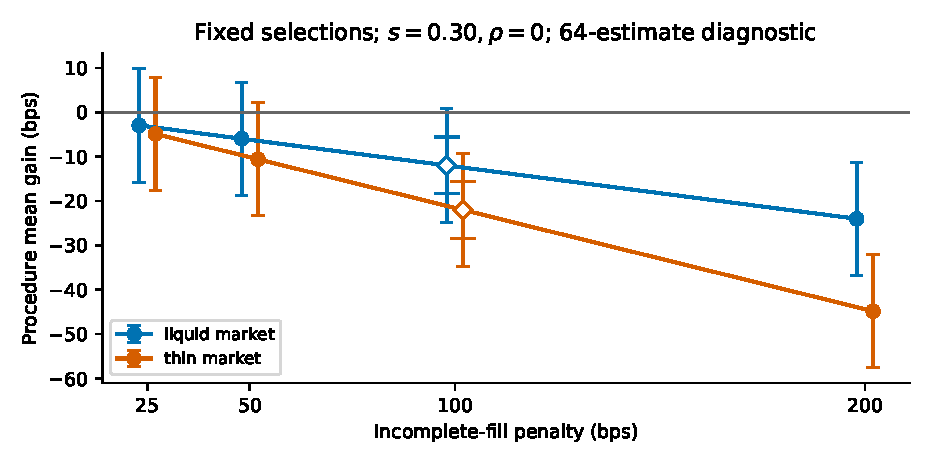
\includegraphics[width=\textwidth,height=0.58\textheight,keepaspectratio]{penalty_sensitivity.pdf}
    \end{column}
    \begin{column}{0.48\textwidth}
      \footnotesize
      \textbf{Post-Outcome Diagnostic Scope}
      \begin{itemize}\itemsep0.18em\parskip0pt
        \item Revalues the \emph{same frozen selected policies} at incomplete-fill penalties $p \in \{25, 50, 100, 200\}$ bps.
        \item Does \textbf{not} reselect candidates under alternative penalties.
        \item The $64$-estimate expanded family, root-deletion audits, alternative simultaneous bands, and break-even analysis are all \textbf{post-outcome diagnostics} separate from the confirmatory $24$-estimate family.
      \end{itemize}
      \vspace{0.2em}
      \begin{block}{Affine break-even diagnostic}
        Uses $\mu(p)=a+p\,b$ with a separate joint component construction. It is descriptive and does \textbf{not} establish a confirmatory threshold.
      \end{block}
    \end{column}
  \end{columns}
\end{frame}

% Frame 12: Auditable deployment assessment report specification
\begin{frame}{Specification for an Auditable Deployment Assessment Report}
  \scriptsize
  To make procedure-level evaluation reproducible and transparent, an assessment report should explicitly separate frozen design choices from post-outcome sensitivity checks:

  \vspace{0.4em}
  \resizebox{0.99\linewidth}{!}{%
  \begin{tabular}{@{}p{0.28\textwidth}p{0.68\textwidth}@{}}
    \toprule
    \textbf{Report Component} & \textbf{Required Specification in This Protocol} \\
    \midrule
    1. Procedure \& Population & Frozen update rule with no-update retention; $50$ roots, $16$ candidates per root, and $100$ root--regime decisions. \\
    \addlinespace[0.25em]
    2. Operating Grid & Explicit environment regimes (liquid, thin), order scales ($s \in \{0.002, 0.05, 0.3\}$), and inventory responses ($\rho \in \{0,1\}$). \\
    \addlinespace[0.25em]
    3. Utility Accounting & Primary $U_{100}$ with a $100$-bps incomplete-fill penalty; $2{,}400$ paired interactive records. \\
    \addlinespace[0.25em]
    4. Unit of Inference & Root-level clustering ($R=50$) recognizing that repeated deployments reduce within-root variance $\sigma_{\text{dep}}^2/(Rm)$ without adding roots. \\
    \addlinespace[0.25em]
    5. Multiplicity Boundary & Strict separation between the prespecified $24$-estimate confirmatory family and post-outcome diagnostics ($64$-estimate family, proxy gap, break-even, root-deletion audits). \\
    \bottomrule
  \end{tabular}
  }
\end{frame}

% Frame 13: Limitations and external validity
\begin{frame}{Limitations and Scope Boundaries}
  \begin{itemize}
    \item \textbf{Single procedure and synthetic market:} All empirical evidence is conditional on one frozen replay-proxy update procedure and one controlled synthetic continuous double auction.
    \item \textbf{Saved-outcome reanalysis:} Current results are a reanalysis of saved outcomes rather than a full raw-model rerun.
    \item \textbf{No broad generalization claims:} The study makes no claim of a universal scaling law, general agent reliability, real-market execution validity, or isolated causal proxy bias.
    \item \textbf{Unmeasured operational dimensions:} Does not measure API monetary cost, token consumption, inference latency, safety constraints, or long-horizon reliability.
    \item \textbf{Auxiliary planner-code case:} The planner-code illustration uses only $3$ generation roots and serves strictly as an auxiliary check, not as statistical evidence for unrestricted coding or autonomous agents.
  \end{itemize}
\end{frame}

% Frame 14: Takeaways and conclusion
\begin{frame}{Takeaways and Conclusion}
  \begin{enumerate}
    \item \textbf{Evaluate the full frozen procedure:} Deployment utility must account for candidate screening, no-update decisions, and interactive feedback at the level of independent generation roots ($R=50$).
    \item \textbf{Scale dominates confirmatory conclusions:} Under the prespecified $24$-estimate family for $U_{100}$, all four largest-scale cells ($s=0.3$) are significantly negative ($-11.98$ to $-22.01$ bps), while smaller scales ($s=0.002, 0.05$) and response contrasts remain unresolved.
    \item \textbf{Proxy gains do not transfer directly:} At the selection scale ($s=0.05$), post-outcome whole-root diagnostics show a positive gap of $0.952$ to $1.314$ bps between saved replay-proxy gains and interactive deployment gains.
    \item \textbf{Completion preferences matter:} Post-outcome revaluation across $25, 50, 100,$ and $200$ bps along the affine frontier $\mu(p) = a + p\,b$ demonstrates how incomplete-fill penalties govern sign and magnitude at large order scales.
    \item \textbf{Disciplined reporting:} Distinguishing prespecified joint confirmatory inference from post-outcome diagnostics prevents overclaiming from multi-condition evaluation suites.
  \end{enumerate}
\end{frame}

\end{document}
